\documentclass{standalone}
\usepackage{tikz}
\usepackage{verbatim}
\begin{document}
\pagestyle{empty}
  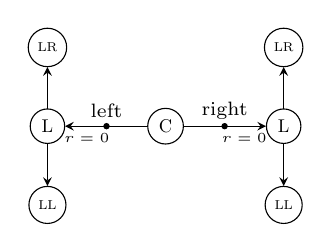
\begin{tikzpicture}
    \node[draw,circle,scale=2/3] (left_right) at (-1.5, 1) {\scriptsize LR};
    \node[draw,circle,scale=2/3] (left_left) at (-1.5, -1) {\scriptsize LL};
    \node[draw,circle,scale=2/3] (left) at (-1.5, 0) {L};
    \node[draw,circle,scale=0.2, fill=black] (al) at (-0.75,0) {};
    \node at (-0.75, 0.2) {\scriptsize left};
    \node at (-1, -0.15) {\tiny $r=0$};
    
    
    \node[draw,circle,scale=2/3] (c) at (+0, 0) {C};
    
    \node[draw,circle,scale=2/3] (right_right) at (1.5, 1) {\scriptsize LR};
    \node[draw,circle,scale=2/3] (right_left) at (1.5, -1) {\scriptsize LL};
    \node[draw,circle,scale=2/3] (right) at (1.5, 0) {L};
    \node[draw,circle,scale=0.2, fill=black] (al) at (0.75,0) {};
    \node at (0.75, 0.2) {\scriptsize right};
    \node at (1, -0.15) {\tiny $r=0$};
    
    \draw[-stealth]  (c) -- (left);
    \draw[-stealth]  (left) -- (left_right);
    \draw[-stealth]  (left) -- (left_left);
    \draw[-stealth]  (c) -- (right);
    \draw[-stealth]  (right) -- (right_right);
    \draw[-stealth]  (right) -- (right_left);
 
  \end{tikzpicture}
\end{document}